\documentclass[10pt]{article}
\usepackage[margin=.76in]{geometry}
\usepackage{amsmath,amssymb,booktabs,microtype,graphicx,float,hyperref,enumitem}
\usepackage[T1]{fontenc}\usepackage{lmodern}
\setlist{nosep,leftmargin=*}\hypersetup{colorlinks=true,linkcolor=blue,urlcolor=blue}
\graphicspath{{results/v4/figures/}{results/v2/figures/}{docs/papers/paper0_6/results/v4/figures/}{docs/papers/paper0_6/results/v2/figures/}}
\title{When Does a Transformer Learn a Reusable Semantic Relation?\\Competence, Depth Extrapolation, and Causal Reuse}
\author{Paper 0.6 --- Semantic / Abstraction Research Line}\date{August 2026}
\begin{document}\maketitle
\begin{abstract}
We distinguish shallow success from a reusable semantic relation by training on trees of depth at most four and testing unseen identities, topologies, path lengths, branching, and distractors. Across 15 Transformer cells (depths 2--12, three seeds), parent, grandparent, $k$-ancestor, and root do not reach held-out competence; \texttt{isAncestor} is stronger but unstable across seeds and model depths. Its deep mean accuracy is 77.62\%, and the minimum cell is 35.42\%. Consequently $L_{\min}(d)$ cannot be estimated and the supported scaling class is threshold failure, not linear or logarithmic composition. Five locally competent \texttt{isAncestor} checkpoints permit bounded causal analysis: intermediate-node masking has negligible effect, root-position masking matters more, and self-attention interventions are more disruptive than feed-forward interventions, favoring a direct membership strategy over path iteration in those cells. A separate competent nested-rule task (S3: 99.93\% mean, 99.22\% worst cell) shows partial causal reuse: matched order-2 donors damage order-3 computation less than unrelated or cross-target donors. The result is a competence-first account: compositional depth can be measurable, but neither shallow accuracy nor geometry licenses a claim that a depth-general predicate was learned.
\end{abstract}

\section{Question and evidential standard}
Let $P(v)$ be the unique parent of a non-root node. We study
\[
 \operatorname{parent}(x)=P(x),\quad \operatorname{grandparent}(x)=P^2(x),\quad
 \operatorname{ancestor}_k(x)=P^k(x),
\]
\[
 \operatorname{isAncestor}(x,y)=\mathbf 1[\exists k\ge1:P^k(x)=y],\qquad
 \operatorname{root}(x)=P^{d(x)}(x).
\]
A learned relation must transfer across unseen token identities and tree topologies and remain competent as total depth $D$, required path $d$, branching $b$, and distractor count $N$ vary independently. Mechanism interpretation is allowed only after an 80\% worst-cell gate. This ordering prevents a representation in an unsuccessful model from being redescribed as semantic computation.

For diagnostic logits $z_\ell$ at residual boundary $\ell$, target margin is
\[m_\ell=z_\ell(y)-\max_{c\ne y}z_\ell(c).\]
For an intervention $I$, we report top-1 change, margin damage $m-m^I$, and Jensen--Shannon damage between output distributions. The stable boundary is the first boundary after which the target remains top-1. These quantities distinguish eventual correctness from when and how the decision is constructed.

\section{Experiments}
\subsection{Predicate phase diagram (S1-v4)}
Training contains depths 2--4 and required hops 1--3. Evaluation uses disjoint query leaves and random unseen topologies at $D\in\{2,3,4,5,6,8,12,16,24,32\}$, hops through 12 where valid, $b\in\{1,2,4,8\}$, $N\in\{0,4,16,64\}$, four templates, and aligned/randomized positions. Internal relation-label vocabulary is shared so test outputs are trained symbols, while queried identities have zero overlap. The phase grid uses width 64, four heads, model depths $L\in\{2,4,6,8,12\}$, and seeds 11, 23, and 37: 15 independently trained cells and 135,360 aggregate evaluation rows.

We define
\[L_{\min}^{(\tau)}(d)=\min\{L:A(L,d,D,b,N)\ge\tau\},\quad \tau\in\{.8,.9\}.
\]
Constant, logarithmic, linear, and sublinear laws are considered only with at least four competent extrapolation points stable over seeds. Otherwise the scientifically meaningful class is threshold failure.

\subsection{Competence-gated causal tests}
Only five \texttt{isAncestor} cells have a deep worst cell at least .8: $(L,s)=(4,23),(6,11),(6,37),(8,11),(12,23)$. For these local successes we decode every path token at every boundary; measure attention to path and off-path tokens; mask parent, intermediate, root, sibling, and distractor positions; zero or mean-replace SA/FF updates; and replace updates or heads with same-role donors from another tree. The other four predicates remain blocked.

\subsection{Three comparison generators}
The earlier controlled suite is retained because it separates kinds of generalization. S1-v2 is explicit in-context taxonomic lookup and passes (98.45\% mean; 85.16\% worst cell). S2 is full-vector relational parity: it reaches essentially zero training loss but only 5.66\% mean and 4.69\% worst-cell held-out accuracy, so all S2 mechanism claims remain blocked. S3 predicts
\[f_1=a_1,\qquad f_2=f_1\oplus a_3,\qquad f_3=f_2\oplus a_6,
\]
and passes unseen combinations (99.93\% mean; 99.22\% worst cell). Its stable decision boundary rises from 1.75 to 2.49 to 4.75 for orders one through three. We now complete its causal test by transplanting order-2 SA/FF updates into order-3 recipients using matched, unrelated same-target, and cross-target donors, plus component and head ablations.

\section{Results: shallow predicate success does not extrapolate}
The phase diagram overturns the tempting interpretation of the easier S1-v2 lookup task. Averaged over the deep regime, accuracies are 7.86\% (parent), 7.72\% (grandparent), 7.57\% (root), 6.52\% ($k$-ancestor), and 77.62\% (\texttt{isAncestor}). Even \texttt{isAncestor} has a 35.42\% minimum cell. The corresponding shallow means are 32.69\%, 31.25\%, 37.22\%, 29.46\%, and 81.86\%. Thus four predicates fail before a depth extrapolation claim can begin; \texttt{isAncestor} displays a mixed basin of local competence rather than seed-stable predicate learning.

\begin{figure}[H]\centering
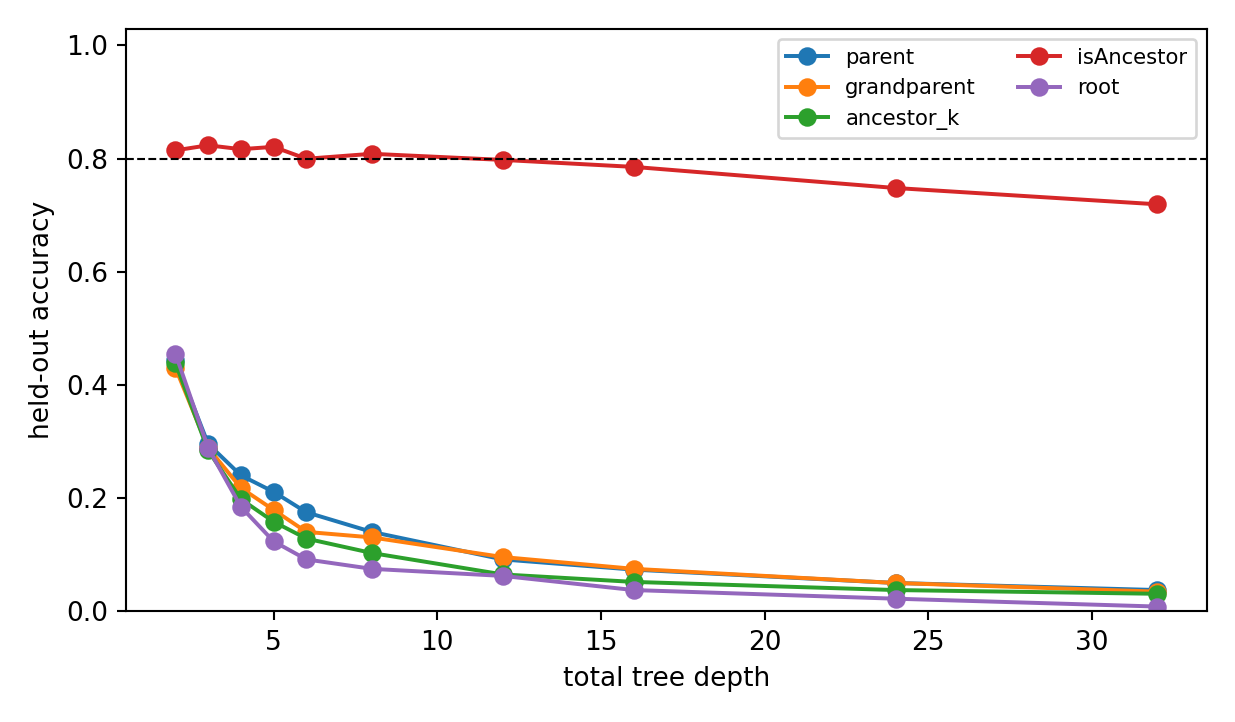
\includegraphics[width=.48\linewidth]{s1_accuracy_vs_tree_depth.png}\hfill
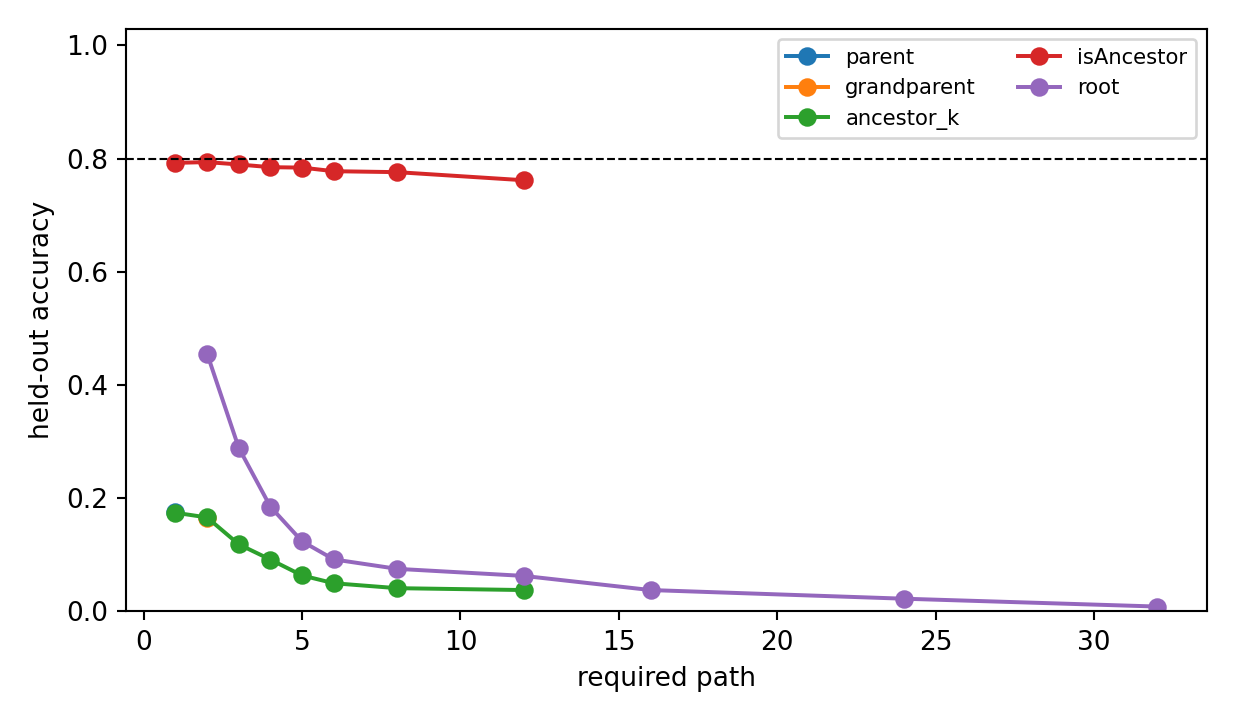
\includegraphics[width=.48\linewidth]{s1_accuracy_vs_required_path.png}
\caption{Held-out predicate accuracy versus total tree depth (left) and required relation path (right). The horizontal line is the competence threshold. Depth and required path are varied explicitly rather than conflated.}\label{fig:depth}
\end{figure}

\begin{figure}[H]\centering
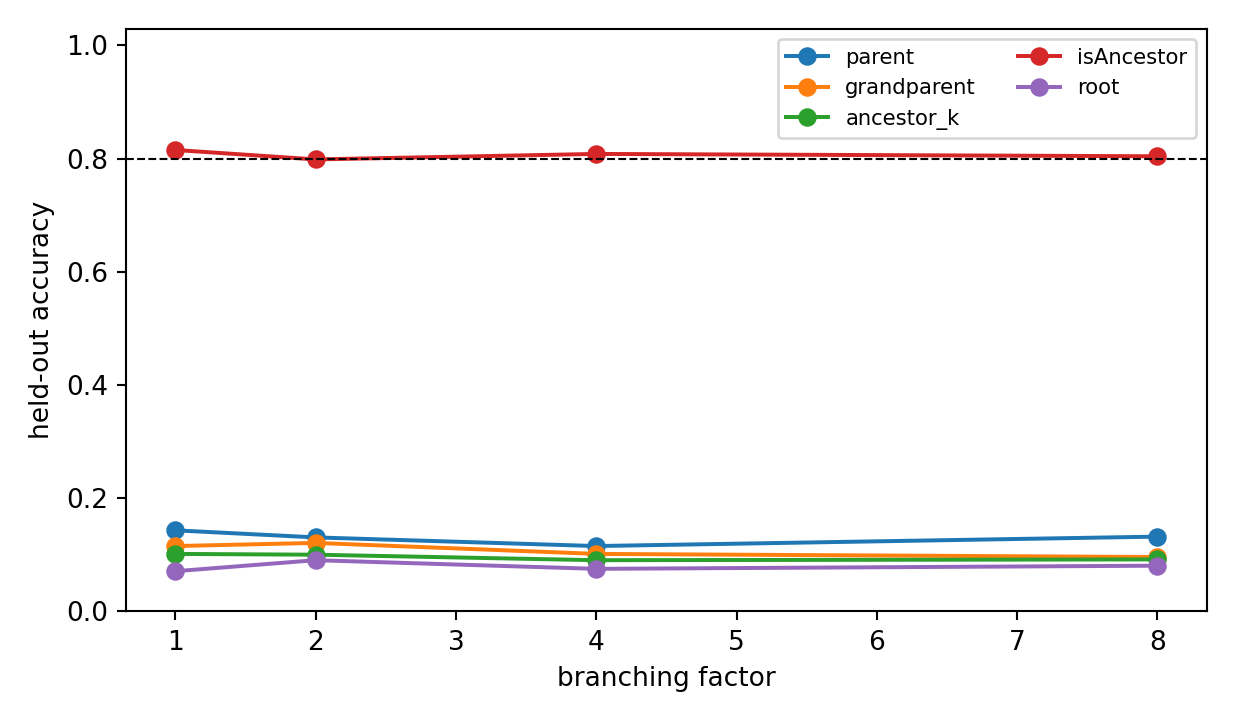
\includegraphics[width=.48\linewidth]{s1_accuracy_vs_branching.png}\hfill
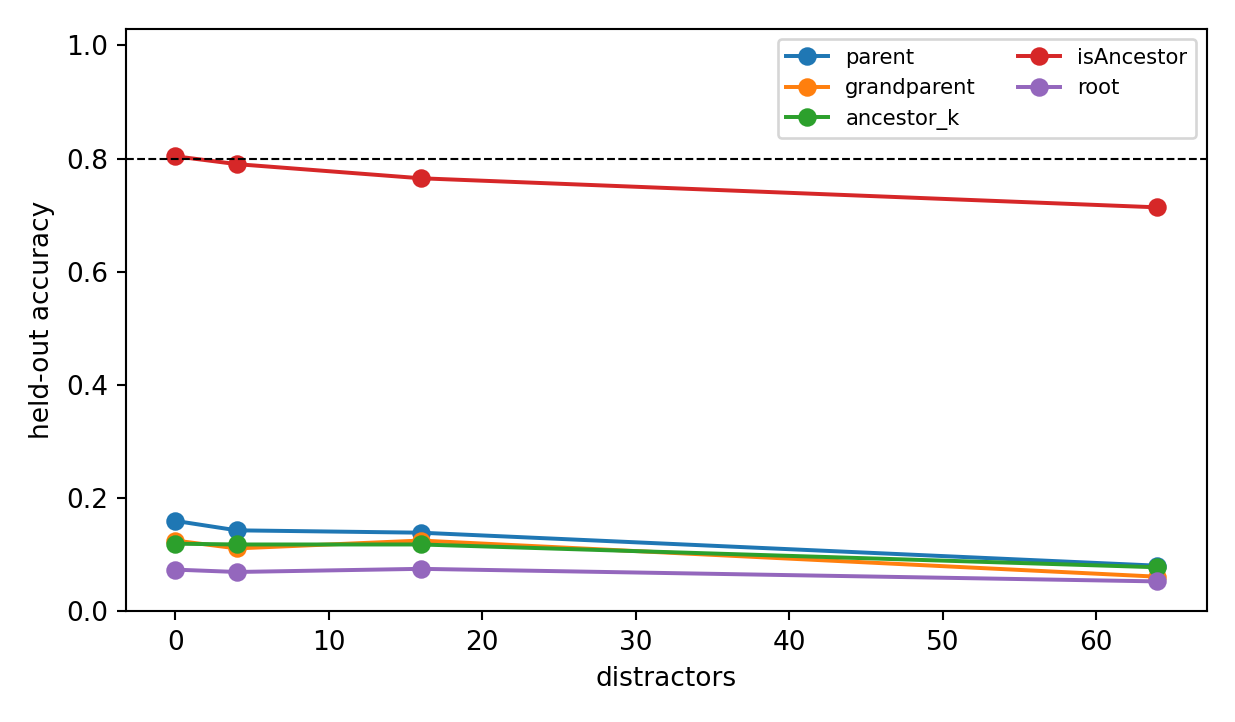
\includegraphics[width=.48\linewidth]{s1_accuracy_vs_distractors.png}
\caption{Independent branching and distractor controls. Neither turns the failed predicates into stable learned relations.}\label{fig:controls}
\end{figure}

\begin{figure}[H]\centering
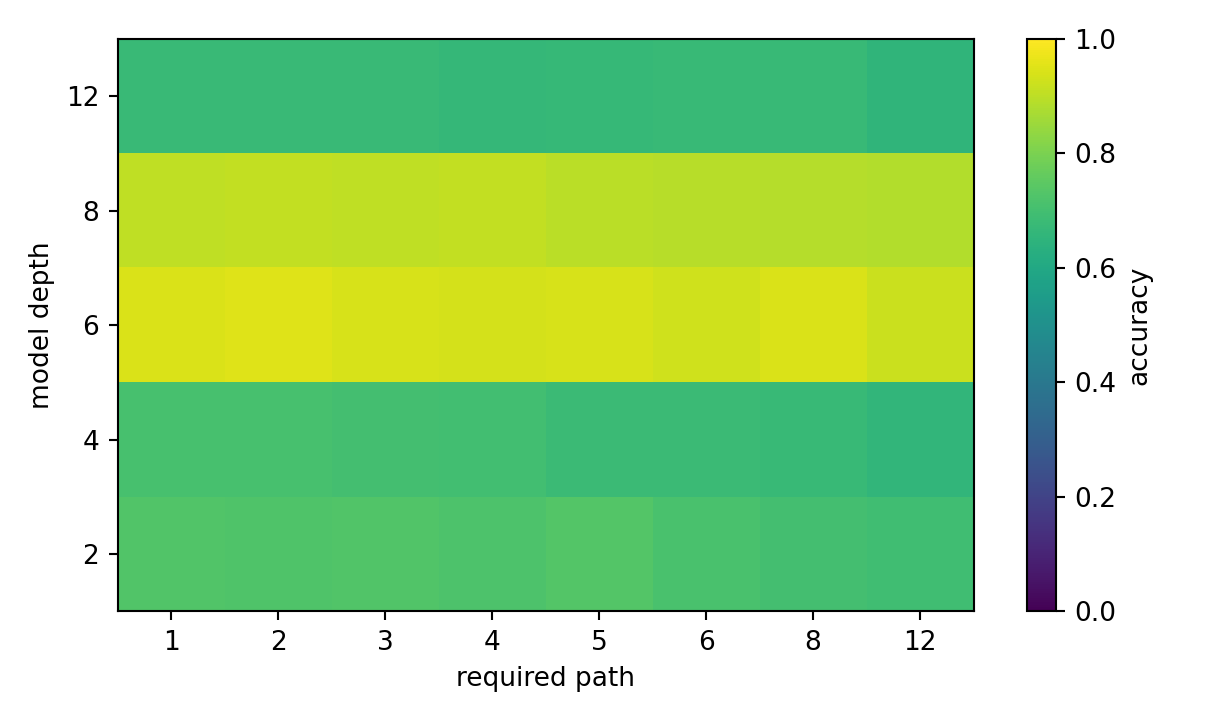
\includegraphics[width=.48\linewidth]{s1_phase_model_depth_vs_path_depth.png}\hfill
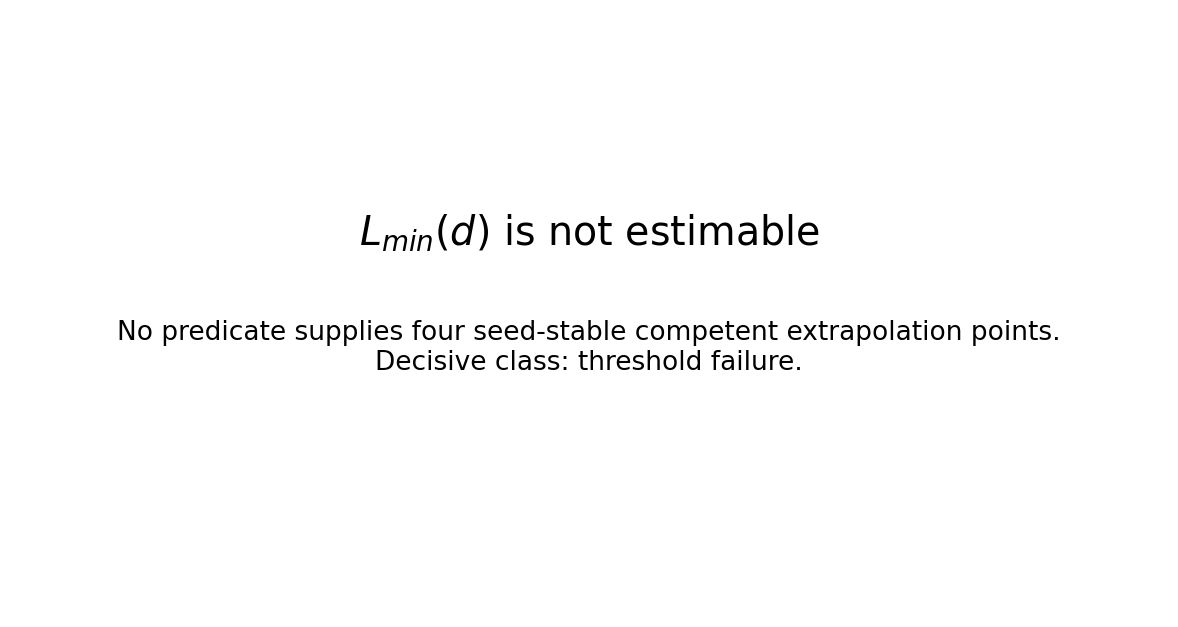
\includegraphics[width=.48\linewidth]{s1_Lmin_scaling_fits.png}
\caption{Left: \texttt{isAncestor} accuracy across model and path depth. Right: why no scaling curve is reported. With fewer than four seed-stable competent extrapolation points, constant, logarithmic, linear, and power fits would be numerically decorative rather than evidence.}\label{fig:phase}
\end{figure}

This is the strong negative outcome anticipated by the protocol: shallow behavior reflects finite-regime interpolation. It is not evidence for one-hop-per-layer iteration, pointer doubling, or constant-depth global execution. In particular, model-depth islands cannot define $L_{\min}(d)$ when adjacent seeds fail the same cell.

\section{Local S1 mechanism: direct membership, not path iteration}
The five competent \texttt{isAncestor} cells are useful local case studies, not a rescue of the central gate. Intermediate-candidate masking produces mean JS damage below $10^{-4}$, whereas masking the root position produces 0.0018. Boundary decoding and attention do not exhibit a stable $1,2,4,8$ hop progression. Together these results favor early/direct endpoint comparison or global membership lookup over a necessary sequential traversal of intermediate ancestors.

\begin{figure}[H]\centering
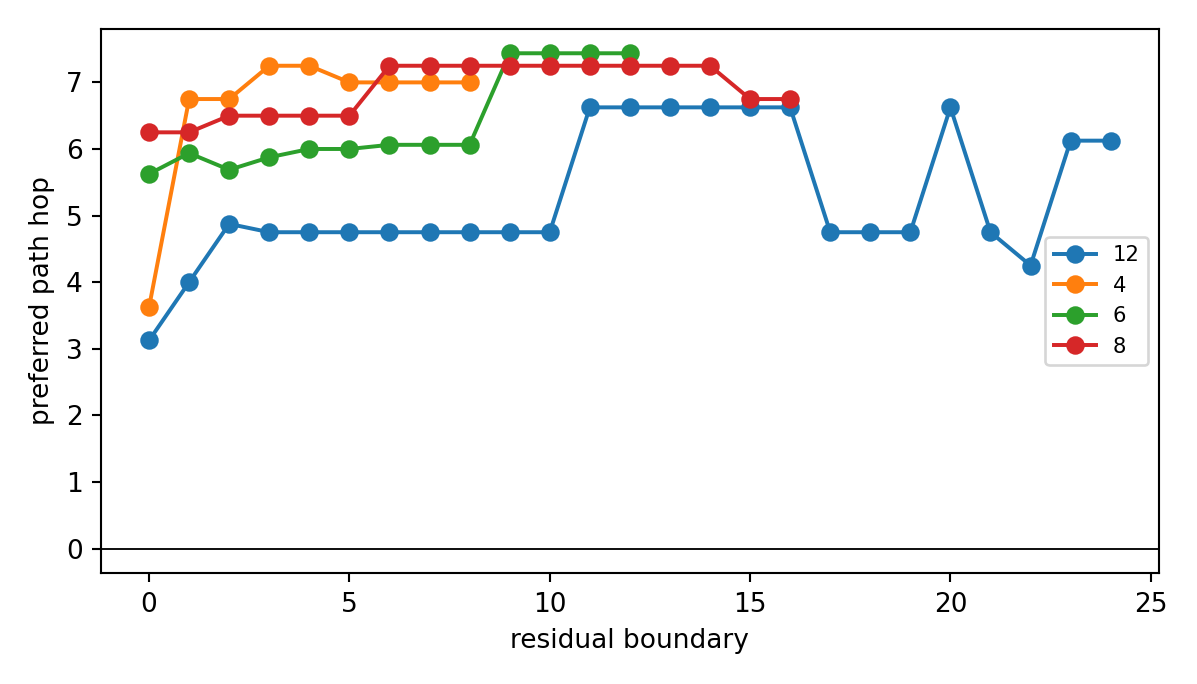
\includegraphics[width=.48\linewidth]{s1_root_intermediate_node_trajectory.png}\hfill
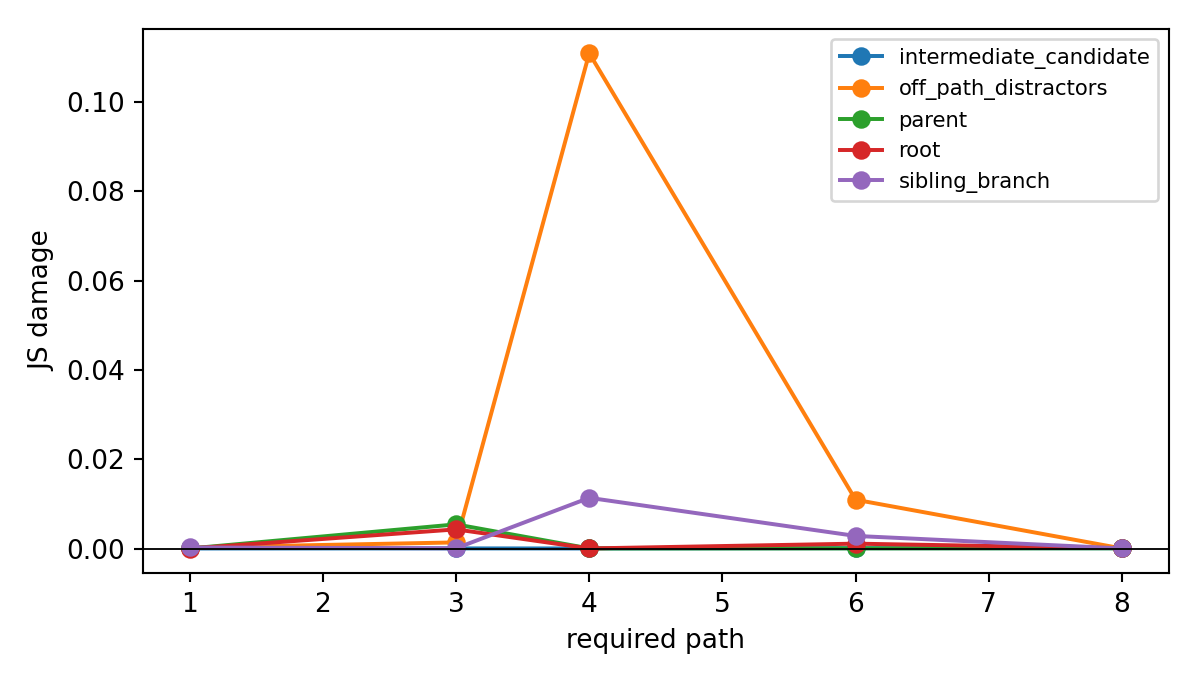
\includegraphics[width=.48\linewidth]{s1_path_masking_effects.png}
\caption{Locally competent \texttt{isAncestor} cells only. Preferred decoded path position (left) lacks a seed-stable iterative trajectory; intermediate masking is nearly harmless compared with endpoint masking (right).}\label{fig:path}
\end{figure}

Same-role cross-tree update replacement causes mean target-margin damage 0.2918: relational role is not freely substitutable across contexts. SA interventions have mean JS damage 0.0619 versus 0.0054 for FF, an approximately eleven-fold contrast. This localizes sensitivity to contextual transport, but does not prove that any individual attention map is an explanation.

\begin{figure}[H]\centering
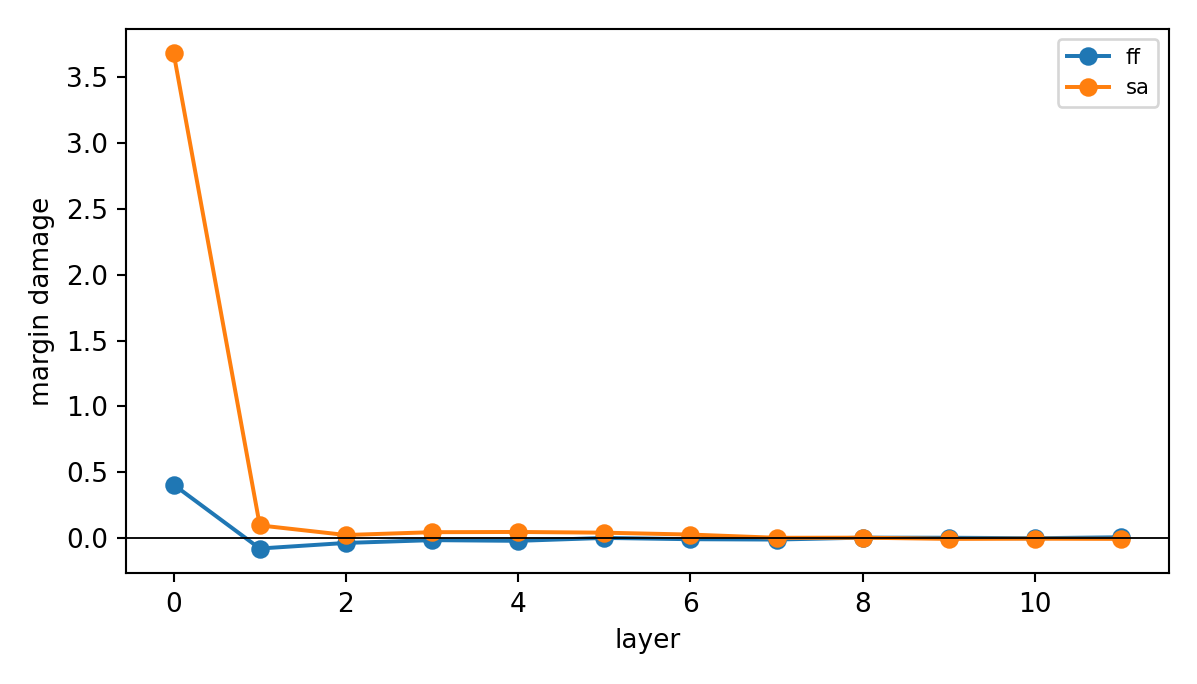
\includegraphics[width=.48\linewidth]{s1_cross_depth_replacement_damage.png}\hfill
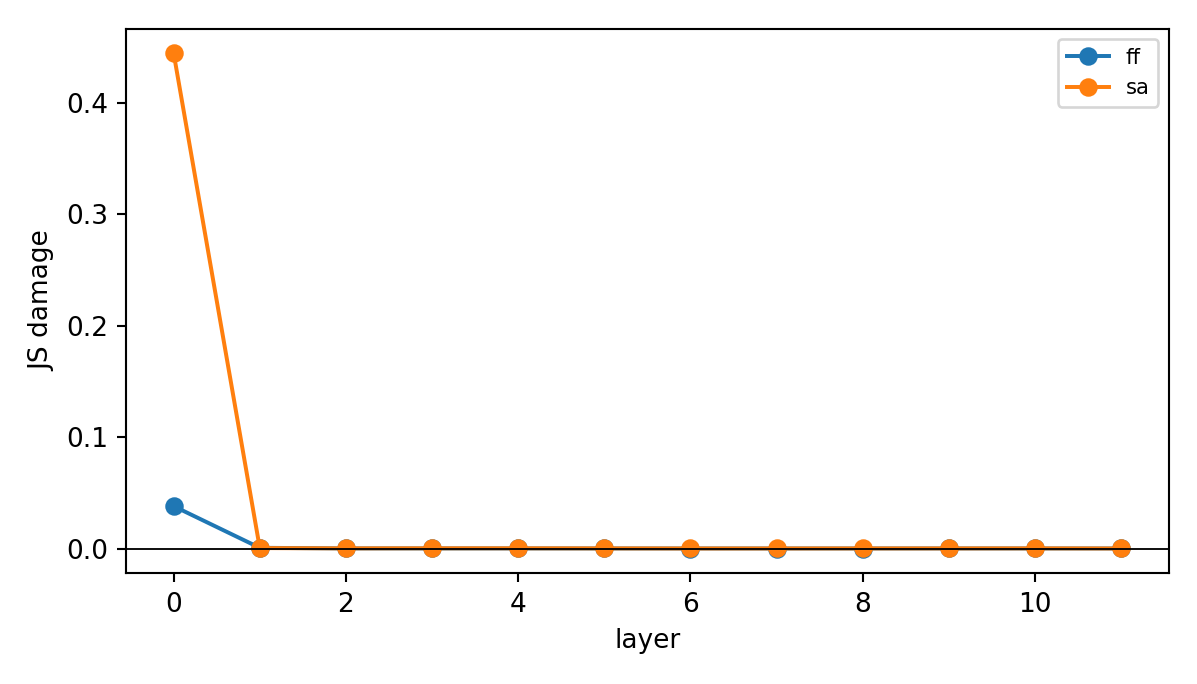
\includegraphics[width=.48\linewidth]{s1_sa_ff_causal_effects.png}
\caption{Cross-tree role replacement (left) and component intervention (right), restricted to competent local cells. SA is substantially more causally sensitive than FF.}\label{fig:s1causal}
\end{figure}

\section{S3 causal reuse of nested computation}
For competent S3, replacing order-3 updates by matched order-2 donors causes mean margin damage 3.6449. An unrelated donor with the same semantic target causes 4.3543, and a cross-target donor causes 6.2256; top-1 flip rates are 12.50\%, 17.19\%, and 23.96\%, respectively. The ordered control matters: target agreement alone does not explain the advantage of matched donors. Order-2 computation is therefore partially reusable inside order-3, although nonzero matched damage shows that the representation remains stage- and context-sensitive.

\begin{figure}[H]\centering
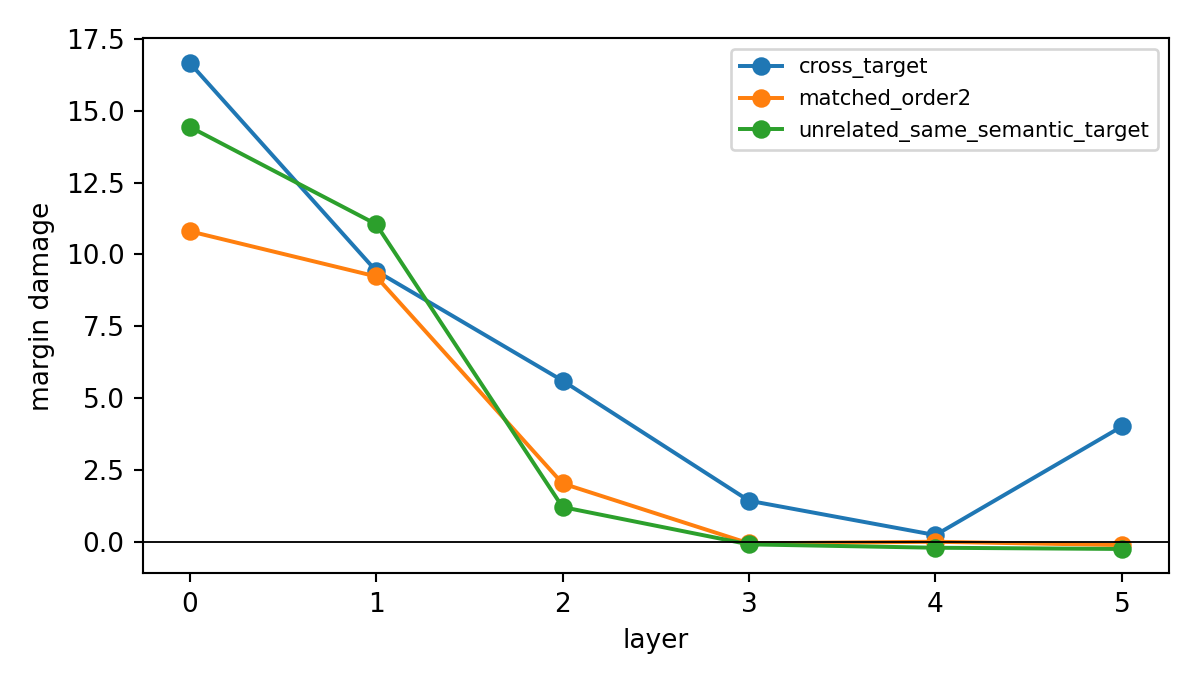
\includegraphics[width=.48\linewidth]{s3_nested_replacement_by_layer.png}\hfill
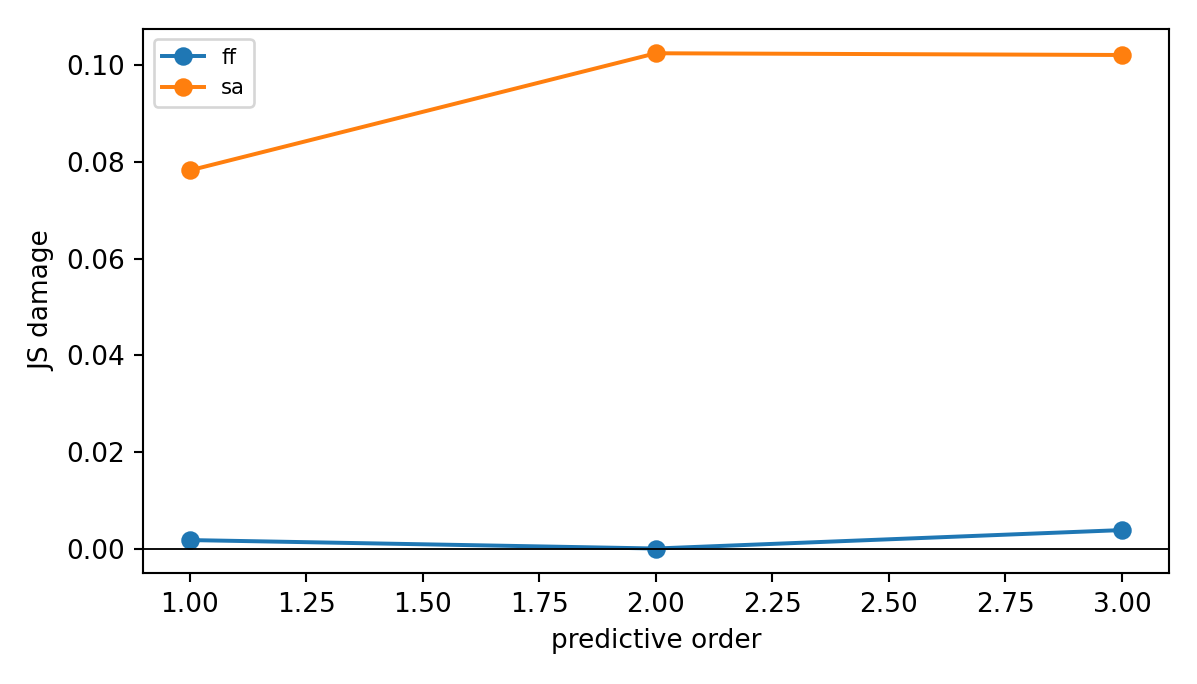
\includegraphics[width=.48\linewidth]{s3_sa_ff_by_predictive_order.png}
\caption{S3 causal completion. Role-matched order-2 donors are less damaging than cross-target controls (left); SA/FF sensitivity changes with predictive order (right).}\label{fig:s3causal}
\end{figure}

The earlier stable-boundary sequence 1.75, 2.49, 4.75 and the donor ordering jointly support a deliberately local theory: more target-relevant composition consumes later computation, partly by reusing lower-order structure. They do not establish a universal hierarchy of semantic abstraction.

\section{Scorecard and interpretation}
No S1-v4 predicate passes most dimensions of the operational scorecard. Identity separation is guaranteed by construction, but parent, grandparent, $k$-ancestor, and root fail held-out topology competence. \texttt{isAncestor} passes locally yet fails seed-stable depth, branching/distractor robustness, and mechanism consistency. Its classification is \emph{mixed, seed-unstable direct membership behavior}; the global classification is threshold failure. S2 remains a memorization negative control. S3 supplies positive evidence for bounded compositional reuse.

The combined lesson is pedagogically simple. First ask whether the rule works beyond its training support. Then ask how the output is constructed. Finally require interventions that distinguish relational role from token identity and target agreement. Reversing this order lets attractive trajectories or clusters assign semantics to a failed computation.

\section{Limitations and reproducibility}
The predicate grid holds width and head count fixed and uses synthetic symbolic relations. Checkpoints are locally reproducible but excluded from version control; all numeric claims are backed by tracked raw CSVs. The configuration is \path{configs/paper06/predicate_v4.json}; generator and model support are in \path{src/cl/semantic/predicates.py} and \path{src/cl/common/model_adapter.py}; phase, causal, and analysis programs are the three \path{paper06_predicate_*.py} modules. Tracked artifacts under \path{results/v4/} include 15-cell competence data, intervention rows, all 16 required figures, scorecard, manifests, and summaries. A broader width/head/training-budget phase is needed before claiming the observed instability is architectural rather than optimization-limited.

\section{Conclusion}
A model can solve explicit taxonomic lookup without learning a predicate that extrapolates in depth. In the harder shallow-train/deep-test instrument, no predicate meets the central seed-stable gate and no scaling law is estimable. Local \texttt{isAncestor} causality favors direct contextual membership over ancestor-by-ancestor iteration. By contrast, competent S3 provides controlled evidence that lower-order computation is partially reused within a higher-order rule. Competence, extrapolation, and causal role invariance are separate requirements; only their conjunction supports a reusable semantic relation.

\appendix
\section{Legacy six-tree pilot}
The original six-tree natural/arbitrary pilot is preserved as a negative control. Across four trained runs its final behavioral accuracy was 1.4--15.3\%, yet post-block normalized separation was 0.110, hierarchy RSA 0.194, and parent-neighbor recovery 0.477 versus 0.254 under permutation. Cross-template cosine reached 0.960. These above-null geometries in an incompetent model motivate the present competence gate. Its 4,320 representation rows, 2,880 component rows, 4,320 entropy rows, 5,760 replacement rows, 2,304 competence rows, 108 aggregates, and 13 figures remain tracked in the legacy artifact tree.

\section{Pretrained and continual-learning boundary}
The pretrained audit remains external-validity material rather than evidence for the controlled claim: training exposure, ontology, and frequencies are unknown. WordNet-style siblings, paraphrase invariance, residual-matched donors, and JVP tests may probe graph recovery but cannot reproduce generator-level counterfactual control. Continual-learning implications are likewise downstream. Failed S2 or unstable S1-v4 features should not be promoted to persistent invariants; competent S3 features are candidates only within the demonstrated generator and causal scope.
\end{document}
